\vspace{1em}
\begin{tcolorbox}
\textbf{Remark} (Previous attempts to scale-up EP) \textbf{.}
As EP appears to be the method of choice for some applications, researchers have attempted to push it to scale. A first approach is to swallow the large computational burden and simply use large data-structures to store the approximating factors (e.g.~TrueSkill \citep{herbrich:trueskill2006}). This approach can only be pushed so far. A second approach is to use the \emph{assumed density filtering} (ADF) algorithm as a simple variant, which only requires a global approximation to be stored \citep{maybeck:adf1982}. ADF, however, provides poorly calibrated uncertainty estimates \citep{minka:ep2001} which was one of the main motivating reasons for developing EP in the first place. 
A third idea, complementary to the one described here, is to use approximating factors that have simpler structure (e.g.~low rank, \citep{qi+minka:sparseGP2010}). This reduces memory consumption (e.g.~for Gaussian factors from $\mathcal{O}(ND^2)$ to $\mathcal{O}(ND)$), but does not stop the scaling with $N$. A fourth idea uses EP to carve up the dataset \citep{gelman:dep2014,xu:sms2014} using approximating factors for collections of data-points. This results in coarse-grained, rather than local, updates and other methods must be used to compute them. (Indeed, the spirit of \cite{gelman:dep2014,xu:sms2014} is to extend sampling methods to large-datasets by exploiting EP's ability to split up inference problems into smaller parts, not EP itself.) 
\end{tcolorbox}

\section{Memory efficient factor tying}

\subsection{A quick comparison between EP and ADF}
%short review on EP
We begin by briefly setting-up the EP and assumed density filtering (ADF) algorithms for posterior approximation, and the readers are referred to Section \ref{sec:chap2_ep_algorithm} for a more detailed review. Recall that EP constructs the approximation $q(\mparam)$ to the exact posterior as the following:\footnote{Here we consider tractable prior distributions, e.g.~Gaussians, otherwise further approximation can be applied and the presented results carry in that case. } 
\begin{equation}
p(\mparam | \data) \approx q(\mparam), \quad p(\mparam | \data) \propto p_0(\mparam) \prod_{n=1}^{N} p(\bm{x}_n | \mparam), \quad q(\mparam) \propto p_0(\mparam) \prod_{n=1}^{N} f_n(\mparam).
\end{equation}
%
The goal of EP is to refine the approximate factors so that they capture the contribution of each of the likelihood terms to the posterior i.e.~$f_n(\mparam) \approx p(\bm{x}_n | \mparam)$. In this spirit, one approach would be to find each approximating factor $f_n(\mparam)$ by minimising the Kullback Leibler (KL) divergence between the posterior and the distribution formed by replacing one of the likelihoods by its corresponding approximating factor,  $\mathrm{KL}[p(\mparam|\data) || p(\mparam|\data) f_n(\mparam)/ p(\bm{x}_n | \mparam)]$. Unfortunately, such an update is still intractable as it involves computing the full posterior. Instead, EP approximates this procedure by replacing the exact leave-one-out posterior $p_{-n}(\mparam) \propto p(\mparam|\data) / p(\bm{x}_n | \mparam)$ on both sides of the KL by the approximate leave-one-out posterior (also called the \emph{cavity} distribution) $q_{-n}(\mparam) \propto q(\mparam)/f_n(\mparam)$. Since this couples the updates for the approximating factors, the updates must now be iterated.

We summarise the update procedure for a single factor in Algorithm \ref{alg:ep}. Critically, the approximation step of EP involves local computations since one likelihood term is treated at a time. The assumption is that these local computations, although possibly requiring further approximation, are far simpler to handle compared to the full posterior $p(\mparam| \data)$. In practice, EP often performs well when the updates are parallelised \citep{microsoft:infernet2014}. Moreover, by using approximating factors for groups of data-points, and then running additional approximate inference algorithms to perform the EP updates (which could include nested EP), EP carves up the data making it suitable for distributed approximate inference.

\begin{figure}[!t]
% UGLY USE OF \vspace & \hspace follows
\begin{minipage}[t]{0.32\linewidth}
\centering
\begin{algorithm}[H] 
\caption{EP} \small
\label{alg:ep} 
\begin{algorithmic}[1] 
	\STATE choose a factor $f_n$ to refine:
	\STATE compute cavity distribution \\$q_{-n}(\mparam) \propto q(\mparam) / f_n(\mparam)$ 
	\STATE compute tilted distribution \\$\tilde{p}_n(\mparam) \propto p(\bm{x}_n|\mparam) q_{-n}(\mparam)$
	\STATE moment matching: \\ \hspace{-5mm}$f_n(\mparam) \leftarrow \mathtt{proj}[\tilde{p}_n(\mparam)] / q_{-n}(\mparam) $
	\STATE inclusion:\\ $q(\mparam) \leftarrow q_{-n}(\mparam) f_n(\mparam)$\\\hspace{1mm}\\ \vspace{1.0mm} \hspace{1mm}\\
\end{algorithmic}
\end{algorithm}
\end{minipage}
%
\begin{minipage}[t]{0.32\linewidth}
\centering
\begin{algorithm}[H] 
\caption{ADF} \small
\label{alg:adf} 
\begin{algorithmic}[1] 
	\STATE choose a datapoint $\bm{x}_n\sim \data$:
	\STATE compute cavity distribution \\$q_{-n}(\mparam) = q(\mparam)$
	\STATE compute tilted distribution \\$\tilde{p}_n(\mparam) \propto p(\bm{x}_n|\mparam) q_{-n}(\mparam)$
	\STATE moment matching: \\ \hspace{-5mm}$f_n(\mparam) \leftarrow \mathtt{proj}[\tilde{p}_n(\mparam)] / q_{-n}(\mparam) $
	\STATE inclusion:\\ $q(\mparam) \leftarrow q_{-n}(\mparam) f_n(\mparam)$\\\hspace{1mm}\\ \vspace{1.0mm} \hspace{1mm}\\
\end{algorithmic}
\end{algorithm}
\end{minipage}
%\quad
\begin{minipage}[t]{0.32\linewidth}
\centering
\begin{algorithm}[H]
\caption{SEP} \small
\label{alg:sep} 
\begin{algorithmic}[1] 
%\STATE initialize $\{\tilde{f}_a\}$
	\STATE choose a datapoint $\bm{x}_n\sim \data$:
	\STATE compute cavity distribution \\ $q_{-1}(\mparam) \propto q(\mparam) / f(\mparam)$
	\STATE compute tilted distribution \\$\tilde{p}_n(\mparam) \propto p(\bm{x}_n|\mparam) q_{-1}(\mparam)$
	\STATE moment matching: \\\hspace{-5mm}$f_n(\mparam) \leftarrow \mathtt{proj}[\tilde{p}_n(\mparam)] / q_{-1}(\mparam) $
	\STATE inclusion:\\ $q(\mparam) \leftarrow q_{-1}(\mparam) f_n(\mparam)$
	\STATE \textit{implicit update}:\\ $f(\mparam) \leftarrow f(\mparam)^{1 - \frac{1}{N}} f_n(\mparam)^{\frac{1}{N}}$
\end{algorithmic}
\end{algorithm}
\end{minipage} 
%
%\caption{Comparing the Expectation Propagation (EP), Assumed Density Filtering (ADF), and Stochastic Expectation Propagation (SEP) update steps. Typically, the algorithms will be initialised using $q(\mparam) = p_0(\mparam)$ and, where appropriate, $f_n(\mparam)=1$ or $f(\mparam)=1$.}
\end{figure}

% ADF
There is, however, one wrinkle that complicates deployment of EP at scale. Computation of the cavity distribution requires removal of the current approximating factor, which means any implementation of EP must store them explicitly necessitating an $\mathcal{O}(N)$ memory footprint. One option is to simply ignore the removal step and replace the cavity distribution with the full approximation, resulting in the assumed density filtering (ADF) algorithm (Algorithm \ref{alg:adf}) \citep{maybeck:adf1982} that only maintains global approximation in memory. But as the moment matching step now over-counts the underlying approximating factor (consider the new form of the objective $\mathrm{KL}[q(\mparam) p(\bm{x}_n | \mparam) || q(\mparam)]$) the variance of the approximation shrinks to zero as multiple passes are made through the dataset. Early stopping, e.g.~after a single pass through the data, is therefore required to prevent overfitting, and generally speaking ADF does not return uncertainties that are well-calibrated to the posterior. 
%
In the next section we introduce a new algorithm that sidesteps EP's large memory demands whilst avoiding the pathological behaviour of ADF. 

\subsection{Stochastic expectation propagation}
%
% SEP
In this section we introduce a new algorithm, inspired by EP, called stochastic expectation propagation (SEP) that combines the benefits of local approximation (tractability of updates, distributability, and parallelisability) with global approximation (reduced memory demands).  The algorithm can be interpreted as a version of EP in which the approximating factors are tied, or alternatively as a corrected version of ADF that prevents overfitting. 
%
The key idea is that, at convergence, the approximating factors in EP can be interpreted as parameterising a global factor,  $f(\mparam)$, that captures the average effect of a likelihood on the posterior  $f(\mparam)^{N} = \prod_{n=1}^{N} f_n(\mparam) \approx \prod_{n=1}^{N} p(\bm{x}_n | \mparam)$. In this spirit, the new algorithm employs direct iterative refinement of a global approximation comprising the prior and $N$ copies of a single approximating factor, $f(\mparam)$, that is $q(\mparam) \propto f(\mparam)^N p_0(\mparam)$.

SEP uses updates that are analogous to EP's in order to refine $f(\mparam)$ in such a way that it captures the \emph{average} effect a likelihood function has on the posterior. First the cavity distribution is formed by removing one of the copies of the factor, $q_{-1}(\mparam) \propto q(\mparam)/f(\mparam)$. 
Second, the corresponding likelihood is included to produce the tilted distribution $\tilde{p}_n(\mparam) \propto q_{-1}(\mparam) p(\bm{x}_n | \mparam)$ and, third, SEP finds an intermediate factor approximation by moment matching, $f_n(\mparam) \leftarrow \mathtt{proj}[\tilde{p}_n(\mparam)] / q_{-1}(\mparam) $. Finally, having updated the factor, it is included into the approximating distribution. It is important here \emph{not} to make a full update since $f_n(\mparam)$ captures the effect of just a single likelihood function  $p(\bm{x}_n | \mparam)$. Instead, damping should be employed to make a partial update $f(\mparam) \leftarrow f(\mparam)^{1 - \epsilon} f_n(\mparam)^{\epsilon}$, and a natural choice uses $\epsilon = 1/N$ which can be interpreted as minimising  $\mathrm{KL}[\tilde{p}_n(\mparam) || p_{0}(\mparam)  f(\mparam)^N]$ in the moment update.

\begin{figure}
\centering
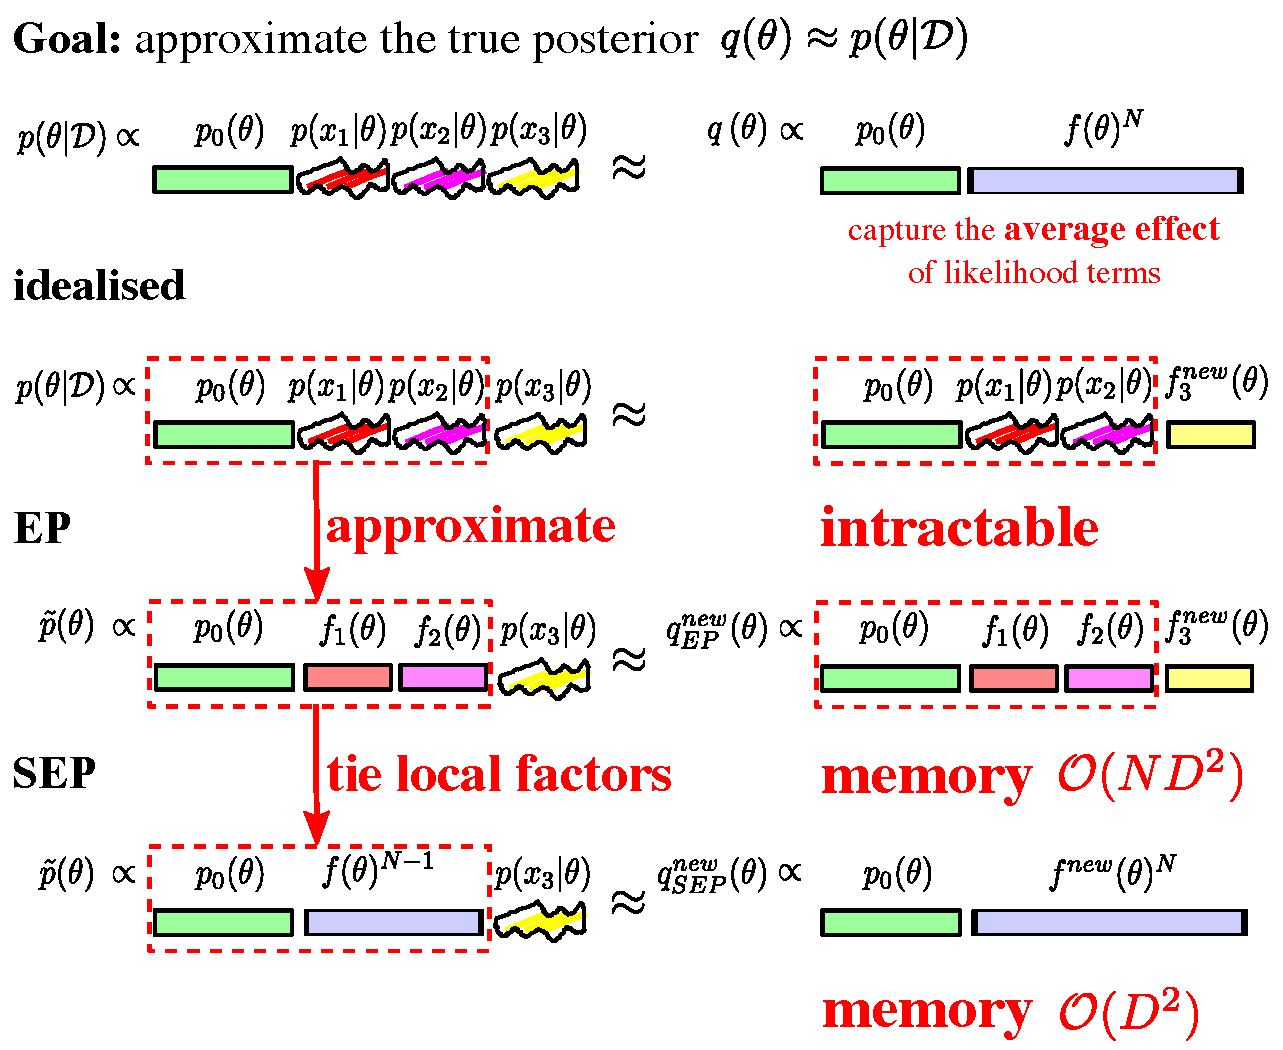
\includegraphics[width=1\linewidth]{Chapter3/sep/fig/algorithm_cartoon}
\caption{A cartoon visualisation for the comparison of three algorithms. Here the boxes represent the prior and the approximating factors, and both of them are assumed to be tractable. The wiggled objects are the complicated likelihood terms to be approximated. An idealised algorithm would approximate each of the likelihood terms given the others fixed as contextual information, which is intractable. EP replaces the ``contextual'' likelihood terms with the approximating factors to form a cavity distribution, making the moment matching step tractable. Finally, SEP ties all the approximating factors, and updates the tied factor by including one randomly sampled likelihood term at each iteration. The space complexity figures are calculated with the assumption of Gaussian approximation.}
\label{fig:chap3_sep_cartoon}
\end{figure}

SEP is summarised in Algorithm \ref{alg:sep}. Unlike ADF, the cavity is formed by dividing out $f(\mparam)$ which captures the average effect of the likelihood and prevents the posterior from collapsing. Like ADF, however, SEP only maintains the global approximation $q(\mparam)$ since $f(\mparam) \propto (q(\mparam) / p_0(\mparam))^{\frac{1}{N}}$ and $q_{-1}(\mparam) \propto q(\mparam)^{1 - \frac{1}{N}} p_0(\mparam)^{\frac{1}{N}}$. When Gaussian approximating factors are used, for example, SEP reduces the storage requirement of EP from  $\mathcal{O}(ND^2)$ to $\mathcal{O}(D^2)$ which is a substantial saving that enables models with many parameters to be applied to large datasets. We also provide a cartoon visualisation for motivating SEP in Figure \ref{fig:chap3_sep_cartoon}.


%


